\clearpage
\chapter{Study Guide 2}

\section{Linear Functions}
\horizontalline{0}{0}

\begin{center}
    \large{\textbf{Study Guide Instructions}}
\end{center}

\horizontalline{-1}{0}

\begin{itemize}
    \item Submit your work in Gradescope as a PDF - you will identify where your “questions are.”
    \item Identify the question number as you submit.  Since we grade "blind" if the questions are NOT identified, the work WILL NOT BE GRADED and a 0 will be recorded. Always leave enough time to 
    identify the questions when submitting.
    \item One section per page (if a page or less) - We prefer to grade the main solution in a single page, extra work can be included on the following page.
    \item Long instructions may be removed to fit on a single page.
    \item \textbf{Do not start a new question in the middle of a page.}
    \item Solutions to book questions are provided for reference.
    \item You may NOT submit given solutions - this includes minor modifications - as your own.
    \item Solutions that do not show individual engagement with the solutions will be marked as no credit and can be considered a violation of honor code.
    \item If you use the given solutions you must reference or explain how you used them, in particular...
\end{itemize}

\horizontalline{-1}{0}

\begin{center}
    \large{\textbf{Method Selection}}
\end{center}

\horizontalline{-1}{0}

\textbf{For full credit,  EACH book exercise in the Study Guides must use one or more of the following methods and FOR EACH QUESTION.  Identify the number the method by number to ensure full credit.}

\begin{itemize}
    \item \textbf{Method 1} - Provide original examples which demonstrate the ideas of the exercise in addition to your solution.
    \item \textbf{Method 2} - Include and discuss the specific topics needed from the chapter and how they relate to the question.
    \item \textbf{Method 3} - Include original Python code, of reasonable length (as screenshot or text)  to show how the topic or concept was explored.
    \item \textbf{Method 4} - Expand the given solution in a significant way, with additional steps and comments. All steps are justified. This is a good method for a proof for which you are only given a basic outline.
    \item \textbf{Method 5} - Attempt the exercise without looking at the solution and then the solution is used to check work. Words are used to describe the results.
    \item \textbf{Method 6} - Provide an analysis of the strategies used to understand the exercise, describing in detail what was challenging, who helped you or what resources were used. The process of understanding is
    described.
\end{itemize}

% Problem 1
\begin{problem}{Problem 1}
    \begin{statement}{Problem Statement}
        Select one page or section of Chapter Two of VMLS to annotate. Include a screenshot of your annotation here.
    \end{statement}

    For this problem I will be using \textbf{Method 2}. \vspace*{1em}

    For this weeks annotation, I have chosen to annotate \textbf{VMLS Section 2.2 - Taylor Approximation}. These annotations can be found on the following pages.

    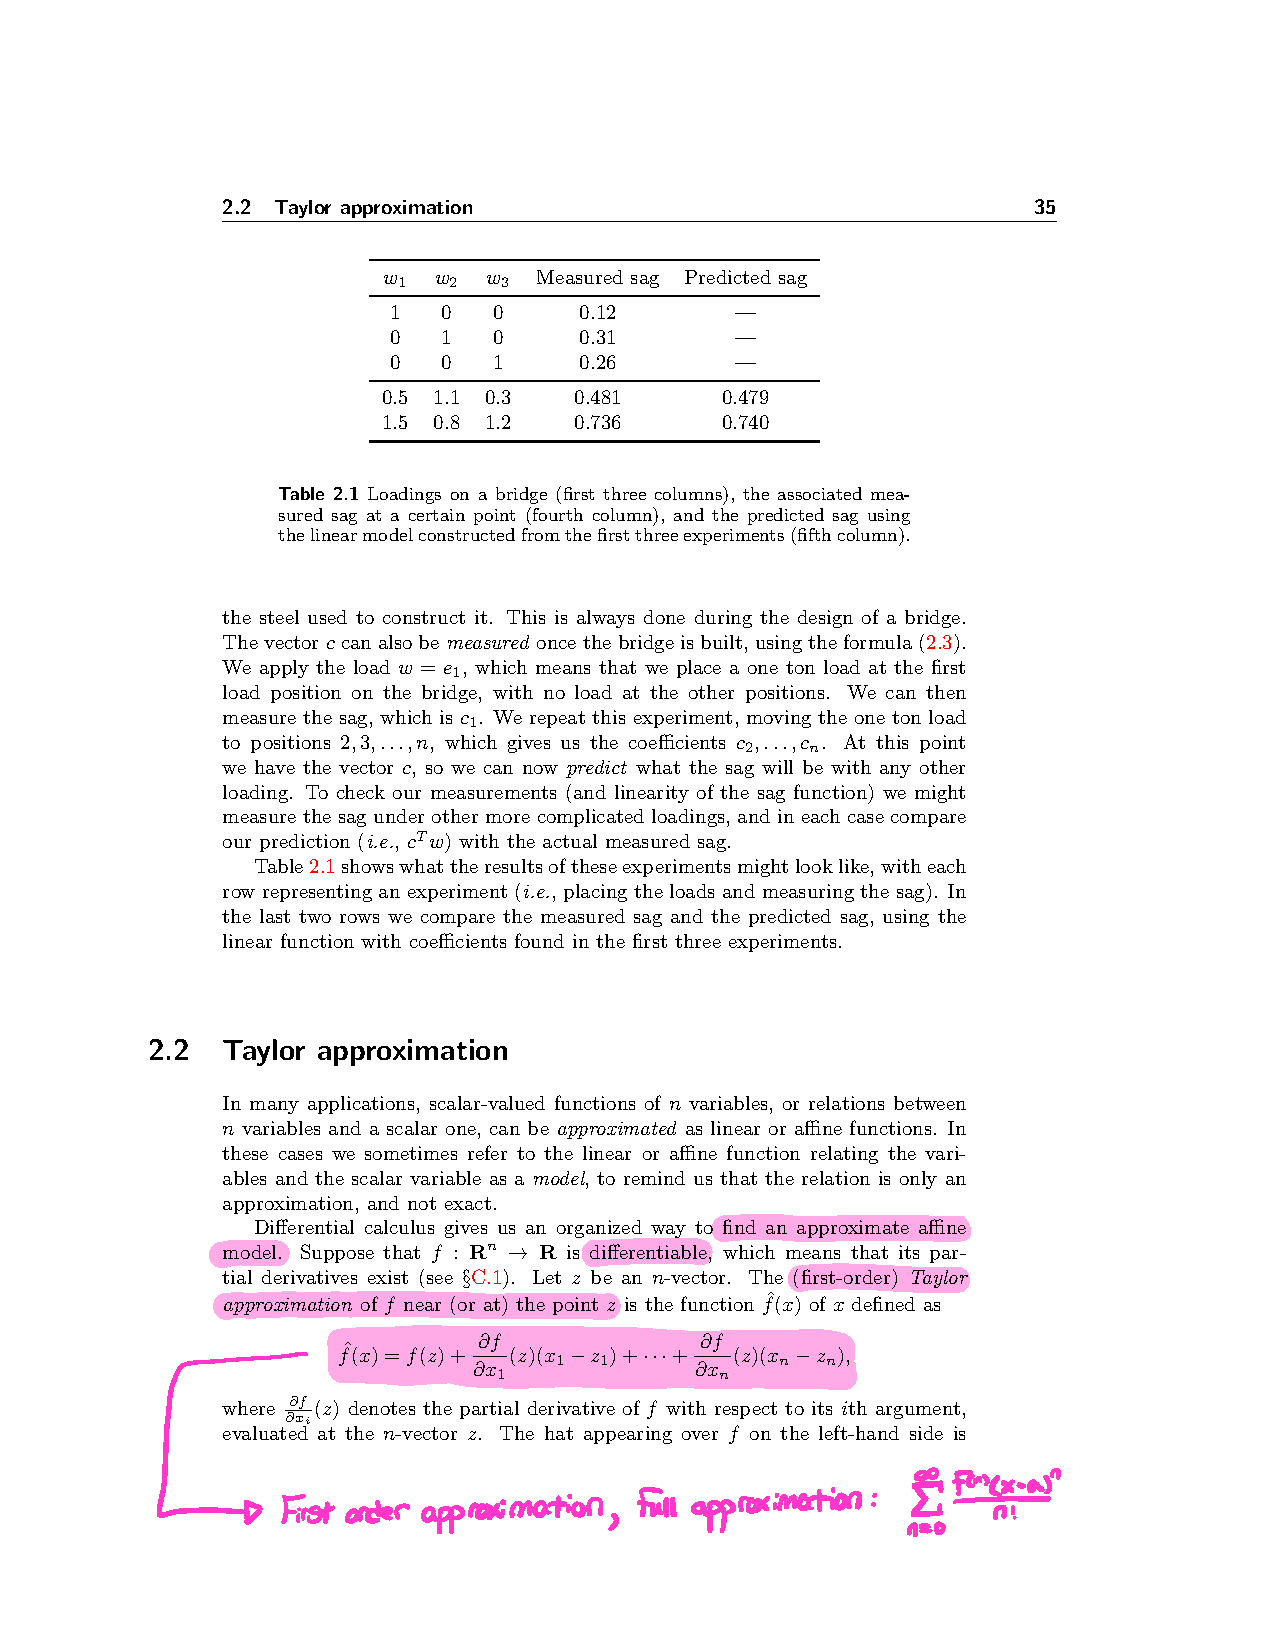
\includepdf[pages={-}, pagecommand={\thispagestyle{fancy}}, width=\paperwidth, offset=0 0]{./PDF/Annotations.pdf}
\end{problem}

% Problem 1 Summary
\begin{summary}{Problem 1 Summary}
    \begin{statement}{Procedure}
        \begin{itemize}
            \item Annotate examples from the chapter that cover the topic of Taylor Series
        \end{itemize}
    \end{statement}
    \begin{statement}{Key Concepts}
        \begin{itemize}
            \item This section covers the topic of what a Taylor series expansion is how it works in the context of linear algebra
        \end{itemize}
    \end{statement}
    \begin{statement}{Variations}
        \begin{itemize}
            \item Since this is a problem is a problem on annotation, the only thing that can change is annotating a different section
        \end{itemize}
    \end{statement}
\end{summary}

% Problem 2
\begin{problem}{Problem 2}
    \begin{statement}{Problem Statement}
        Solve the Chapter 2 Random exercise from the video and Piazza in your own words here. \vspace*{1em}

        \textbf{Original Question} \vspace*{1em}

        \textit{General formula for affine functions.} Verify that formula (2.4) holds for any affine function $f:\mathbf{R}^{n}\rightarrow\mathbf{R}$. You can use the fact that $f(x) = a^{T}x + b$ for some $n$-vector $a$ 
        and scalar $b$.
    \end{statement}

    \begin{highlight}[Solution]
        For this problem, I will be using \textbf{Method 4}. \vspace*{1em}

        The formula that is referenced in the problem statement (2.4) is 

        \setcounter{equation}{0}
        \begin{equation}
            f(x) = f(0) + x_{1}(f(e_{1}) - f(0)) + \dots + x_{n}(f(e_{n}) - f(0)) = f(0) + \sum^{n}_{i = 1} x_{i}(f(e_{i}) - f(0)).
        \end{equation}

        We know that by definition 

        \begin{equation}
            f(x) = a^{T}x + b,
        \end{equation}
        this implies that $f(0)$ is going to result in an inner product of $a$ with the zero vector. This means we can say that $f(0)$ is then

        \begin{equation}
            f(0) = a^{T}\mathbf{0} + b = 
            \begin{bmatrix}
                a_{1} & \dots & a_{n}
            \end{bmatrix}
            \begin{bmatrix}
                0 \\
                \vdots \\
                0 \\
            \end{bmatrix}
            + b = 0(a_{1}) + \dots + 0(a_{n}) + b = b.
        \end{equation}
        From equation (3) we see that $f(0)$ is just the scalar value $b$. We now aim to express the other terms in equation (1). Starting with the general form $x_{n}(f(e_{n}) - f(0))$ we can first
        define $f(e_{n})$ to be

        \begin{equation}
            f(e_{n}) = a^{T}e_{n} + b = 
            \begin{bmatrix}
                a_{1} & \dots & a_{n}
            \end{bmatrix}
            \begin{bmatrix}
                0 \\
                \vdots \\
                1 \\
            \end{bmatrix}
            + b = a_{1}(0) + \dots + a_{n}(1) + b = a_{n}(1) + b = a_{n} + b.
        \end{equation}
        In equation (4), $e_{n}$ is the $n^{\text{th}}$ basis vector (a vector filled with zeros for elements with the exception of the $n^{\text{th}}$ element is a 1). Combining equation (4) with the 
        result from (3) we can justifiably say that $f(e_{n}) - f(0)$ is thus

        \begin{equation}
            f(e_{n}) - f(0) = a_{n} + b - b = a_{n}.
        \end{equation}
        This in turn implies that $x_{n}(f(e_{n}) - f(0))$ is

        \begin{equation}
            x_{n}(f(e_{n}) - f(0)) = x_{n}a_{n}.
        \end{equation}
        We can further say from the result of equation (6) that

        \begin{equation}
            f(x) = f(0) + \sum^{n}_{i = 1} x_{i}(f(e_{i}) - f(0)) = b + \sum^{n}_{i = 1} x_{i}a_{i} = b + a^{T}x = a^{T}x + b.
        \end{equation}
        We used the commutative property to re-arrange our final result to match the definition of $f(x)$ as well as the commutative property of inner products to say $\sum^{n}_{i=1}x_{i}a_{i} = a^{T}x$.
        Consequently (2.4) holds for any affine function.
    \end{highlight}
\end{problem}

% Problem 2 Summary
\begin{summary}{Problem 2 Summary}
    \begin{statement}{Procedure}
        \begin{itemize}
            \item Take the formula (2.4) from the problem statement and show that the zero vector evaluates to the scalar $b$
            \item Take the same formula (2.4) from the problem statement and show that it evaluates to $a_{n} + b$ for the unit vector $(e_{n})$
            \item Show what the term $f(e_{n}) - f(0)$ evaluates to
            \item Show what the term $x_{n}(f(e_{n}) - f(0)) = x_{n}a_{n}$ evaluates to
            \item Piece together the following terms to show what the formula evaluates to
        \end{itemize}
    \end{statement}
    \begin{statement}{Key Concepts}
        \begin{itemize}
            \item Affine functions are of the form $f(x) = a^{T}x + b$
            \item Formula (2.4) has the form $f(x) = f(0) + \sum^{n}_{i = 1} x_{i}(f(e_{i}) - f(0)) = a^{T}x + b$ for any affine function
        \end{itemize}
    \end{statement}
    \begin{statement}{Variations}
        \begin{itemize}
            \item We could be asked to show that an affine function would hold for a different formula
            \begin{itemize}
                \item We would then have to go through the same procedure to show that it holds
            \end{itemize}
        \end{itemize}
    \end{statement}
\end{summary}

% Problem 3
\begin{problem}{Problem 3}
    \begin{statement}{Problem Statement}
        Explain the solution to 2.1 here in your own words. (Since you are given a solution, you will be graded on your ability to explain). \vspace*{1em}

        \textbf{Original Question} \vspace*{1em}

        \textit{Linear} or \textit{not}? Determine whether each of the following scalar-valued functions of $n$-vectors is linear. If it is a linear function, give its inner product representation, 
        i.e., an $n$-vector a for which $f(x)=a^{T}x$ for all $x$. If it is not linear, give specific $x, y, \alpha,$ and $\beta$ for which superposition fails, i.e.,

        \begin{equation*}
            f(\alpha x + \beta y) \neq \alpha f(x) + \beta f(y).
        \end{equation*}

        \begin{enumerate}[label=(\alph*)]
            \item The spread of values of the vector, defined as $f(x) = \text{max}_{k}x_{k} - \text{min}_{k}x_{k}$.
            \item The difference of the last element and the first, $f(x) = x_{n}-x_{1}$.
            \item The median of an $n$-vector, where we will assume $n = 2k + 1$ is odd. The median of the vector $x$ is defined as the $(k+1)^{\text{st}}$ largest number among the entries of $x$.
            For example, the median of $(-7.1,3.2,-1.5)$ is $(-1.5)$.
            \item The average of the entries with odd indices, minus the average of the entries with even indices. You can assume that $n = 2k$ is even.
            \item Vector extrapolation, defined as $x_{n} + (x_{n}-x_{n-1})$, for $n \geq 2$. (This is a simple prediction of what $x_{n+1}$ would be, based on a straight line drawn through $x_{n}$
            and $x_{n-1}$.)
        \end{enumerate}
    \end{statement}

    \begin{highlight}[Solution - Part (a)]
        For this problem, I will be using \textbf{Method 4}. \vspace*{1em}

        Function for this part: $f(x) = \text{max}_{k}x_{k} - \text{min}_{k}x_{k}$. \vspace*{1em}

        \textbf{\textit{VMLS Solution:}} \vspace*{1em}

        \textit{Not linear.} Choose $x = (1,0), y = (0,1), \alpha = \beta = 1/2$. Then $\alpha x + \beta y = (1/2,1/2)$, $f(x) = f(y) = 1$, and
        
        \setcounter{equation}{0}
        \begin{equation}
            f(\alpha x + \beta y) = 0 \neq \alpha f(x) + \beta f(y) = 1.
        \end{equation}

        \textbf{\textit{Explanation:}} \vspace*{1em}

        The fundamental reason as to why this function is not linear is because there exists a given set of vectors that will cause superposition (the addition of two vectors into one) to fail. In this
        example, the authors chose the vectors $x = (1,0)$ and $y = (0,1)$ along with $\alpha = \beta = 1/2$ to demonstrate this point. When we calculate the minimum value being subtracted from the maximum
        value of a given vector, it can be shown that 

        \begin{equation}
            f(\alpha x + \beta y) = f \Bigg( \frac{1}{2} \cdot
                \begin{bmatrix}
                    1 \\
                    0 \\
                \end{bmatrix}
                + \frac{1}{2} \cdot
                \begin{bmatrix}
                    0 \\
                    1 \\
                \end{bmatrix} 
                \Bigg) = 
                f \Bigg ( 
                \begin{bmatrix}
                    \frac{1}{2} \\
                    0 \\
                \end{bmatrix}
                + 
                \begin{bmatrix}
                    0 \\
                    \frac{1}{2} \\
                \end{bmatrix}
                \Bigg) = f \Bigg(
                \begin{bmatrix}
                    \frac{1}{2} \\
                    \frac{1}{2} \\
                \end{bmatrix}
                \Bigg) = \text{max} - \text{min} = 1/2 - 1/2 = 0.
        \end{equation}
        Where, if we now try to test the law of superposition to prove that this specific example is linear we have

        \begin{equation}
            f(x) = f \Bigg(
                \begin{bmatrix}
                    1 \\
                    0 \\
                \end{bmatrix}
                \Bigg) = \text{max} - \text{min} = 1 - 0 = 1 \hspace*{5pt} , \hspace*{5pt}
            f(y) = f \Bigg(
                \begin{bmatrix}
                    1 \\
                    0 \\
                \end{bmatrix}
                \Bigg) = \text{max} - \text{min} = 1 - 0 = 1
        \end{equation}
        where we then calculate 

        \begin{equation}
            \alpha f(x) + \beta f(y) = \frac{1}{2}(1) + \frac{1}{2}(1) = 1 \hspace*{5pt} \rightarrow \hspace*{5pt} f(\alpha x + \beta y) \neq \alpha f(x) + \beta f(y) \hspace*{5pt} \rightarrow \hspace*{5pt} 1 \neq 0
        \end{equation}
        and thus superposition fails and this is not linear.
    \end{highlight}

    \begin{highlight}[Solution - Part (b)]
        For this problem, I will be using \textbf{Method 4}. \vspace*{1em}

        Function for this part: $f(x) = x_{n} - x_{1}$. \vspace*{1em}

        \textbf{\textit{VMLS Solution:}} \vspace*{1em}

        \textit{Linear}. The function can be written as an inner product $f(x) = a^{T}x$ for 

        \begin{equation}
            a = (-1, 0, \dots , 0, 1).
        \end{equation}

        \textbf{\textit{Explanation:}} \vspace*{1em}

        The simplest explanation for why this is indeed linear is that when calculating the difference between the first and last element of a vector, there is no scalar value ($\alpha , \beta$) that when applied to the vectors
        that will cause the difference between the scaled vector and original vector to be different. Namely 

        \begin{equation}
            f(\alpha x + \beta y) = \alpha (x_{n}) - \alpha (x_{1}) + \beta (y_{n}) - \beta (y_{1}) = \alpha (x_{n} - x_{1}) + \beta (y_{n} - y_{1}) = \alpha f(x) + \beta f(y).
        \end{equation}
        Equation (6) satisfies superposition and thus this function is indeed linear. This vector would then be represented as 

        \begin{equation}
            a = 
            \begin{bmatrix}
                - 1 \\
                0 \\
                \vdots \\
                0 \\
                1 \\
            \end{bmatrix}
        \end{equation}
        where the middle elements must be zero so that we end up with $f(x) = x_{n} - x_{1}$ for our function. 
    \end{highlight}

    \begin{highlight}[Solution - Part (c)]
        For this problem, I will be using \textbf{Method 4}. \vspace*{1em}

        Function for this part: Median of vector. \vspace*{1em}

        \textbf{\textit{VMLS Solution:}} \vspace*{1em}

        \textit{Not linear}. Choose $x = (-1,0,3), y = (2,-1,0), \alpha = \beta = 1$. Then $\alpha x + \beta y = (1,-1,2), f(x) = f(y) = 0,$ and

        \begin{equation}
            f(\alpha x + \beta y) = 1 \neq \alpha f(x) + \beta f(y) = 0.
        \end{equation}

        \textbf{\textit{Explanation:}} \vspace*{1em}

        This function fails superposition and is not linear. In this example, we are grabbing the median value (which is the second largest element in a vector by the problems definition)
        of a given vector. It can be shown for this specific example that there exists an $\alpha$ and $\beta$ such that superposition will fail and thus the function will be non linear.
        In our case, with the values that the other chose for the vectors we see that

        \begin{equation}
            f(x) = f \Bigg(
                \begin{bmatrix}
                    -1 \\
                    0 \\ 
                    3 \\
                \end{bmatrix}
                \Bigg) = 0 \hspace*{5pt} , \hspace*{5pt}
            f(y) = f \Bigg(
                \begin{bmatrix}
                    2 \\
                    - 1 \\
                    0 \\
                \end{bmatrix}
                \Bigg) = 0 \hspace*{5pt} \rightarrow \hspace*{5pt} \alpha f(x) + \beta f(y) = 1(0) + 1(0) = 0.
        \end{equation}
        Consequently, it can also be shown that with $\alpha = \beta = 1$ that

        \begin{equation}
            f(\alpha x + \beta y) = f \Bigg(
                1 \cdot 
                \begin{bmatrix}
                    - 1 \\
                    0 \\
                    3 \\
                \end{bmatrix}
                + 1 \cdot 
                \begin{bmatrix}
                    2 \\
                    -1 \\
                    0 \\
                \end{bmatrix}
                \Bigg) = f \Bigg(
                \begin{bmatrix}
                    1 \\
                    -1 \\
                    3 \\
                \end{bmatrix}
                \Bigg ) = 1.
        \end{equation}
        By the law of superposition we have just shown $f(\alpha x + \beta y) \neq \alpha f(x) + \beta f(y)$ and thus this function is not linear.
    \end{highlight}

    \begin{highlight}[Solution - Part (d)]
        For this problem, I will be using \textbf{Method 4}. \vspace*{1em}

        Function for this part: Average of odd indices minus average of even indices. \vspace*{1em}

        \textbf{\textit{VMLS Solution:}} \vspace*{1em}

        \textit{Linear}. If the size of the vector is even ($n = 2m$), there are $m$ even and $m$ odd indices, and $f(x) = a^{T}x$ with

        \begin{equation}
            a = (1/m, -1/m, 1/m, -1/m, \dots, 1/m, -1/m).
        \end{equation}

        \textbf{\textit{Explanation:}} \vspace*{1em}

        This function passes superposition and is thus linear. If we write out the function in mathematical terms, we have

        \begin{equation}
            f(x) = \frac{1}{k} \Bigg(\sum_{i = i,3,\dots, 2k-1} x_{i} - \sum_{i = 2,4,\dots, 2k} x_{i}\Bigg)
        \end{equation}
        and no matter the value of $\alpha$ and $\beta$ we can show

        \begin{equation}
            f(\alpha x + \beta y) = \alpha f(x) + \beta f(y)
        \end{equation}
        and the function will scale linearly. This vector is scaled with a factor of the value $k$ and is thus represented as

        \begin{equation}
            a = 
            \begin{bmatrix}
                1/k \\
                -1/k \\
                \vdots \\
                1/k \\
                -1/k \\
            \end{bmatrix}
        \end{equation}
        where when a scalar value is applied to this vector, the averages of the odd and even indices will scale accordingly.
    \end{highlight}

    \begin{highlight}[Solution - Part (e)]
        For this problem, I will be using \textbf{Method 4}. \vspace*{1em}

        Function for this part: Vector extrapolation ($x_{n} + (x_{n} - x_{n-1})$) for $n \geq 2$. \vspace*{1em}

        \textbf{\textit{VMLS Solution:}} \vspace*{1em}

        \textit{Linear}. We have $f(x) = a^{T}x$ for 
        
        \begin{equation}
            a = (0,0,\dots,0,-1,2).
        \end{equation}

        \textbf{\textit{Explanation:}} \vspace*{1em}

        This function is linear because it satisfies the law of superposition. For any given value of $\alpha$ or $\beta$ the scaled vector will match the combination of scaled vectors independently.
        For instance, if we choose $x = (0,1,2)$ and $y = (-1,1,3)$ with $\alpha = \beta = 1$

        \begin{equation}
            f(\alpha x + \beta y) = f \Bigg(
                1 \cdot 
                \begin{bmatrix}
                    0 \\
                    1 \\
                    2 \\
                \end{bmatrix}
                + 1 \cdot 
                \begin{bmatrix}
                    -1 \\
                    1 \\
                    3 \\
                \end{bmatrix}
                \Bigg) = f \Bigg(
                \begin{bmatrix}
                    -1 \\
                    2 \\
                    5 \\
                \end{bmatrix}
                \Bigg) = 8.
        \end{equation}
        Consequently, for this specific example we can show

        \begin{equation}
            \alpha f(x) + \beta f(y) = 1 \cdot f \Bigg(
                \begin{bmatrix}
                    0 \\
                    1 \\
                    2 \\
                \end{bmatrix}
                \Bigg) + 1 \cdot f \Bigg(
                \begin{bmatrix}
                    -1 \\
                    1 \\
                    3 \\
                \end{bmatrix}
                \Bigg) = 1(3) + 1(5) = 8
        \end{equation}
        and thus

        \begin{equation}
            f(\alpha x + \beta y) = \alpha f(x) + \beta f(y).
        \end{equation}
        Although equations (16) through (18) are for a specific example, any arbitrary set of vectors ($x,y$) with any arbitrary scalar values ($\alpha,\beta$) will satisfy the law of superposition
        and thus the function is linear. For the inner product representation of this function, we constitute that $a$ must be

        \begin{equation}
            a = 
            \begin{bmatrix}
                0 \\
                \vdots \\
                -1 \\
                2 \\
            \end{bmatrix}.
        \end{equation}
        We require the trailing elements in $a$ to be zero so that when the inner product of $a$ is taken with $x$ we get the resulting function $f(x) = x_{n} + (x_{n} - x_{n-1}) = 2x_{n} - x_{1}$.
        The scalar values (-1,2) are chosen for the last elements of $a$ such that when the inner product is carried out with an arbitrary vector $x$, we get the previous expression.
    \end{highlight}
\end{problem}

% Problem 3 Summary
\begin{summary}{Problem 3 Summary}
    \begin{statement}{Procedure}
        \begin{enumerate}[label = (\alph*)]
            \item Part (a)
            \begin{itemize}
                \item Pick two vectors that can disprove the law of superposition
                \item Go through the machinery of the law of superposition for the given function of the problem
            \end{itemize}
            \item Part (b)
            \begin{itemize}
                \item Go through the machinery of the law of superposition for the given function of the problem
                \item Show that the law of superposition holds for this specific function
            \end{itemize}
            \item Part (c)
            \begin{itemize}
                \item Pick two vectors that can disprove the law of superposition
                \item Go through the machinery of the law of superposition for the given function of the problem
            \end{itemize}
            \item Part (d)
            \begin{itemize}
                \item Go through the machinery of the law of superposition for the given function of the problem
                \item Show that the law of superposition holds for this specific function
            \end{itemize}
            \item Part (e)
            \begin{itemize}
                \item Go through the machinery of the law of superposition for the given function of the problem
                \item Show that the law of superposition holds for this specific function
            \end{itemize}
        \end{enumerate}
    \end{statement}
    \begin{statement}{Key Concepts}
        \begin{itemize}
            \item For a function to be considered linear, it must be of the form 
            \begin{equation*}
                f(\alpha x + \beta y) = \alpha f(x) + \beta f(y)
            \end{equation*}
            for all values of $\alpha$ and $\beta$
        \end{itemize}
    \end{statement}
    \begin{statement}{Variations}
        \begin{itemize}
            \item We could be given a different function to prove it is linear or not
            \begin{itemize}
                \item Go through the same machinery of reasoning if the law of superposition holds for a given function
            \end{itemize}
        \end{itemize}
    \end{statement}
\end{summary}

% Problem 4
\begin{problem}{Problem 4}
    \begin{statement}{Problem Statement}
        Explain the solution to 2.4 here in your own words. (Since you are given a solution, you will be graded on your ability to explain). \vspace*{1em}

        \textbf{Original Question} \vspace*{1em}

        \textit{Linear function?} The function $\phi$: $\mathbf{R}^{3} \rightarrow \mathbf{R}$ satisfies

        \begin{equation*}
            \phi(1,1,0) = -1, \hspace*{10pt} \phi(-1,1,1) = 1, \hspace*{10pt} \phi(1,-1,-1) = 1.
        \end{equation*}
        Choose one of the following, and justify your chose: $\phi$ must be linear; $\phi$ could be linear; $\phi$ cannot be linear.
    \end{statement}

    \begin{highlight}[Solution]
        For this problem, I will be using \textbf{Method 4}. \vspace*{1em}

        \textbf{\textit{VMLS Solution:}} \vspace*{1em}

        The correct answer is: $\phi$ \textit{cannot be linear}. To see this, we note that the third point $(1,-1,-1)$ is the negative of the second point $(-1,1,1)$. If $\phi$ were linear,
        the two values of $\phi$ would need to be negatives of each other. But they are 1 and 1, not negatives of each other. \vspace*{1em}

        \textbf{\textit{Explanation:}} \vspace*{1em}

        For the mapping of a function from one space to another, it must satisfy \textit{homogeneity} and \textit{additivity}. We first check additivity to show

        \setcounter{equation}{0}
        \begin{equation}
            \phi(x + y) = \phi \Bigg(
                \begin{bmatrix}
                    1 \\
                    1 \\
                    0 \\
                \end{bmatrix}
                + 
                \begin{bmatrix}
                    1 \\
                    -1 \\
                    -1 \\
                \end{bmatrix}
                \Bigg) = \phi \Bigg(
                \begin{bmatrix}
                    2 \\
                    0 \\
                    -1 \\
                \end{bmatrix}
                \Bigg) \hspace*{5pt} , \hspace*{5pt}
            \phi(x + y) = \phi \Bigg(
                \begin{bmatrix}
                    1 \\
                    1 \\
                    0 \\
                \end{bmatrix}
                +
                \begin{bmatrix}
                    -1 \\
                    1 \\
                    1 \\
                \end{bmatrix}
                \Bigg) = \phi \Bigg(
                \begin{bmatrix}
                    0 \\
                    2 \\
                    1 \\
                \end{bmatrix}
                \Bigg)
        \end{equation}
        that these functions $\phi$ fail the additivity property. This is because the resulting functions that are produced after using the additivity property do not exist in this space that we are 
        provided. Therefore the additivity property cannot be confirmed. (Due to the associativity property of vector sums I do not need to show the other combinations, the result will be the same.)

        We can then check the homogeneity property with ($\alpha = -1$) of these functions and show

        \begin{align}
            \phi(\alpha x) & = \phi \Bigg(
                -1 \cdot 
                \begin{bmatrix}
                    1 \\
                    1 \\
                    0 \\
                \end{bmatrix}
                \Bigg) = \phi \Bigg(
                \begin{bmatrix}
                    -1 \\
                    -1 \\
                    0 \\
                \end{bmatrix}
                \Bigg) = ? \neq \alpha \phi(x) = (-1) \phi(1,1,0) = 1 \\
            \phi(\alpha x) & = \phi \Bigg(
                -1 \cdot 
                \begin{bmatrix}
                    -1 \\
                    1 \\
                    1 \\
                \end{bmatrix}
                \Bigg) = \phi \Bigg(
                \begin{bmatrix}
                    1 \\
                    -1 \\
                    -1 \\
                \end{bmatrix}
                \Bigg) = 1 \neq \alpha \phi(x) = (-1) \phi(-1,1,1) = -1  \\
            \phi(\alpha x) & = \phi \Bigg(
                -1 \cdot 
                \begin{bmatrix}
                    1 \\
                    -1 \\
                    -1 \\
                \end{bmatrix}
                \Bigg) = \phi \Bigg(
                \begin{bmatrix}
                    -1 \\
                    1 \\
                    1 \\
                \end{bmatrix}
                \Bigg) = 1 \neq \alpha \phi(x) = (-1)\phi(1,-1,-1) = -1
        \end{align}
        that these functions do not satisfy homogeneity and cannot be linear functions.
    \end{highlight}
\end{problem}

% Problem 4 Summary
\begin{summary}{Problem 4 Summary}
    \begin{statement}{Procedure}
        \begin{itemize}
            \item For the functions that are presented to us, test them with the homogeneity and additivity principle
            \item Test two of the functions with the additivity principle and show that the resulting function does not exist in this space
            \item Choose a value for $\alpha$ and show that it doesn't hold for the homogeneity principle
        \end{itemize}
    \end{statement}
    \begin{statement}{Key Concepts}
        \begin{itemize}
            \item For a function to be considered linear, they must follow the following principles
            \begin{align*}
                f(\alpha x) & = \alpha f(x) & \text{(Homogeneity)} \\
                f(x + y) & = f(x) + f(y) & \text{(Additivity)}
            \end{align*}
            \item These functions that are presented to us are not considered linear because they do not uphold the homogeneity and additivity principle
            \item The additivity principle fails because the resulting function does not have a value in this space
        \end{itemize}
    \end{statement}
    \begin{statement}{Variations}
        \begin{itemize}
            \item We could be given different functions to prove if they are linear or not
            \begin{itemize}
                \item In this case we would use the homogeneity and additivity principle to test if the functions are linear or not
            \end{itemize}
        \end{itemize}
    \end{statement}
\end{summary}

% Problem 5
\begin{problem}{Problem 5}
    \begin{statement}{Problem Statement}
        Explain the solution to 2.6 here in your own words. (Since you are given a solution, you will be graded on your ability to explain). \vspace*{1em}

        \textbf{Original Question} \vspace*{1em}

        \textit{Questionnaire Scoring.} A questionnaire in a magazine has 30 questions, broken into two sets of 15 questions. Someone taking the questionnaire answers each question with `Rarely',
        `Sometimes', or `Often'. The answers are recorded as a 30-vector $a$, with $a_{i} = 1,2,3$ if question $i$ is answered Rarely, Sometimes, or Often, respectively. The total score on a completed
        questionnaire is found by adding up 1 point for every question answered Sometimes and 2 points for every question answered Often on questions 1-15, and by adding 2 points and 4 points for those
        responses on questions 16-30. (Nothing is added to the score for Rarely responses.) Express the total score $s$ in the form of an affine function $s = w^{T}a + v$ where $w$ is a 30-vector and $v$
        is a scalar (number).
    \end{statement}

    \begin{highlight}[Solution]
        For this problem, I will be using \textbf{Method 4}. \vspace*{1em}

        \textbf{\textit{VMLS Solution:}} \vspace*{1em}

        We have $w = (\mathbf{1}_{15},2\mathbf{1}_{15})$ and $v = -45$. The contribution to the score from questions 1-15 is given by $\mathbf{1}^{T}(a_{1:15}-\mathbf{1})$. The contribution to the scores 
        from questions 16-30 is given by $2\mathbf{1}^{T}(a_{16:30}-\mathbf{1})$. So, we can write the overall score as

        \setcounter{equation}{0}
        \begin{equation}
            (\mathbf{1}_{15},2\mathbf{1}_{15})^{T}(a-\mathbf{1}) = (\mathbf{1}_{15},2\mathbf{1}_{15})^{T}a - 45.
        \end{equation}

        \textbf{\textit{Explanation:}} \vspace*{1em}

        For starters, the term ($a-\mathbf{1}$) represents a 30 vector that is used to create the desired representation of the responses for each question. Here, if the participant responds with `Rarely' 
        then this element will be 0 (1 - 1) (since $\mathbf{1}$ is a vector of 1's in every entry), `Sometimes' will evaluate to 1 (2 - 1) and `Often' will evaluate to 2 (3 - 1). The term $(\mathbf{1}_{15},2\mathbf{1}_{15})^{T}$
        is another 30 vector that represents the weighting of the first 15 and last 15 questions respectively. Putting this together we get a representation of the total score from the responses with

        \begin{equation}
            s = (\mathbf{1}_{15},2\mathbf{1}_{15})^{T}(a-\mathbf{1}).
        \end{equation}
        
        Now, to make this function affine we must add a constant scalar value to the end of our inner product. For the first 15 entries, we are subtracting a value of 1 from each element and for the last 
        15 we are subtracting 2 from each element. This simplifies to $-1(15) - 2(15) = -45$, this is how we obtain the value of $v$ to be $-45$. We can simplify the equation in equation (1) to then just 
        take the inner product of the weighted responses for both the first 15 and last 15 responses of the survey with the scoring values found in $a$. Since the first 15 questions are weighted with a factor
        of just 1, we have the term ($\mathbf{1}_{15}$) and since the last 15 responses are weighted with a value of 2, we have the term ($2\mathbf{1}_{15}$). Stitching this together to get an affine function
        we have

        \begin{equation}
            s = (\mathbf{1}_{15},2\mathbf{1}_{15})^{T}a - 45.
        \end{equation}
        Equations (2) and (3) are equivalent where equation (3) represents an affine function.
    \end{highlight}
\end{problem}

% Problem 5 Summary
\begin{summary}{Problem 5 Summary}
    \begin{statement}{Procedure}
        \begin{itemize}
            \item Generate a term that can accurately depict the responses for the questionnaire (this is represented by subtracting the value 1 from each entry)
            \item Generate a vector that will accurately represent the weighting of the questions from the questionnaire (this is done by concatenating a 10 vector with a 20 vector)
            \item Write an expression that encapsulates each of these terms in the form of an inner product
            \item To create an equivalent expression to the previous one, subtract the scalar 45 from the inner product of the weighting of the responses and the answers from the questionnaire
        \end{itemize}
    \end{statement}
    \begin{statement}{Key Concepts}
        \begin{itemize}
            \item This problem shows that an inner product can be written as an affine function with correct manipulation of the original inner product
        \end{itemize}
    \end{statement}
    \begin{statement}{Variations}
        \begin{itemize}
            \item We could be given a different question that encapsulates a different scenario and asked to do a similar operation
            \begin{itemize}
                \item We then would use similar methods to show that the inner product could be represented as an affine function
            \end{itemize}
        \end{itemize}
    \end{statement}
\end{summary}

% Problem 6
\begin{problem}{Problem 6}
    \begin{statement}{Problem Statement}
        \begin{enumerate}[label=(\alph*)]
            \item Re-do the proof on page 30 that an inner product satisfies superposition with 2 vectors of your own choosing (using length 3).
            \item Is this still a proof?
            \item Why is it useful?
        \end{enumerate}
    \end{statement}

    \begin{highlight}[Solution - Part (a)]
        For this problem, I will be using \textbf{Method 1}. \vspace*{1em}

        To do this proof, we first define arbitrary vectors for ($x,y,a$) and scalar values ($\alpha,\beta$)

        \setcounter{equation}{0}
        \begin{equation}
            x =
            \begin{bmatrix}
                x_{1} \\
                x_{2} \\
                x_{3} \\
            \end{bmatrix}
            \hspace*{5pt} , \hspace*{5pt}
            y = 
            \begin{bmatrix}
                y_{1} \\
                y_{2} \\
                y_{3} \\
            \end{bmatrix}
            \hspace*{5pt} , \hspace*{5pt}
            a = 
            \begin{bmatrix}
                a_{1} \\
                a_{2} \\
                a_{3} \\
            \end{bmatrix}.
        \end{equation}
        Starting with $f(\alpha x + \beta y) = a^{T}(\alpha x + \beta y)$ we can show
        
        \begin{align}
            f(\alpha x + \beta y) & = 
            \begin{bmatrix}
                a_{1} & a_{2} & a_{3} \\
            \end{bmatrix}
            \Bigg(
            \alpha \cdot 
            \begin{bmatrix}
                x_{1} \\
                x_{2} \\
                x_{3} \\
            \end{bmatrix}
            + \beta \cdot
            \begin{bmatrix}
                y_{1} \\
                y_{2} \\
                y_{3} \\
            \end{bmatrix}
            \Bigg) \\
            & = 
            \begin{bmatrix}
                a_{1} & a_{2} & a_{3} \\
            \end{bmatrix}
            \Bigg(
            \begin{bmatrix}
                \alpha x_{1} + \beta y_{1} \\
                \alpha x_{2} + \beta y_{2} \\
                \alpha x_{3} + \beta y_{3} \\
            \end{bmatrix}
            \Bigg) \\
            & = a_{1}(\alpha x_{1} + \beta y_{1}) + a_{2}(\alpha x_{2} + \beta y_{2}) + a_{3}(\alpha x_{3} + \beta y_{3}) \\
            & = a_{1} \alpha x_{1} + a_{1} \beta y_{1} + a_{2} \alpha x_{2} + a_{2} \beta y_{2} + a_{3} \alpha x_{3} + a_{3} \beta y_{3} \\
            & = \alpha(a_{1}x_{1} + a_{2}x_{2} + a_{3}x_{3}) + \beta(a_{1}y_{1} + a_{2}y_{2} + a_{3}y_{3}) \\
            & = \alpha (a^{T}x) + \beta (a^{T}y) \\
            & = \alpha f(x) + \beta f(y).
        \end{align}
        To get to equation (8), we used the definition of an inner product, namely $f(k) = a^{T}k$ where $k$ is an arbitrary vector (in our case $x$ and $y$).

        If we would like to show an example of this with actual values and not just placeholders for values, we would need to show equivalence between equation (5) (or equation (6)) and equation (7) 
        (or equation (8)). For this example, we will define our vectors to be 

        \begin{equation}
            x =
            \begin{bmatrix}
                1 \\
                2 \\
                3 \\
            \end{bmatrix}
            \hspace*{5pt} , \hspace*{5pt}
            y = 
            \begin{bmatrix}
                4 \\
                5 \\
                6 \\
            \end{bmatrix}
            \hspace*{5pt} , \hspace*{5pt}
            a = 
            \begin{bmatrix}
                a_{1} \\
                a_{2} \\
                a_{3} \\
            \end{bmatrix}
            \hspace*{5pt} , \hspace*{5pt} 
            (\alpha , \beta)
        \end{equation}
        First we use equation (5), when we do this we obtain

        \footnotesize
        \begin{align}
            a_{1} \alpha x_{1} + a_{1} \beta y_{1} + a_{2} \alpha x_{2} + a_{2} \beta y_{2} + a_{3} \alpha x_{3} + a_{3} \beta y_{3} & = a_{1} \alpha (1) + a_{1} \beta (4) + a_{2} \alpha (2) + a_{2} \beta (5) + a_{3} \alpha (3) + a_{3} \beta (6) \\
            & = \alpha (a_{1} + 2a_{2} + 3a_{3}) + \beta (4a_{1} + 5a_{2} + 6a_{3}) 
        \end{align}

        Now, for superposition to hold for our given example we require equation (11) to be equal to that of the result that will come out of equation (7). Carrying out the steps for equation (7)
        we find

        \normalsize
        \begin{align}
            \alpha(a^{T}x) + \beta(a^{T}y) & = \alpha \cdot
            \Bigg(
            \begin{bmatrix}
                a_{1} & a_{2} & a_{3} \\
            \end{bmatrix}
            \begin{bmatrix}
                1 \\
                2 \\
                3 \\
            \end{bmatrix}
            \Bigg) + \beta \cdot
            \Bigg(
            \begin{bmatrix}
                a_{1} & a_{2} & a_{3} \\
            \end{bmatrix}
            \begin{bmatrix}
                4 \\
                5 \\
                6 \\
            \end{bmatrix}
            \Bigg) \\
            & = \alpha(a_{1} + 2a_{2} + 3a_{3}) + \beta(4a_{1} + 5a_{2} + 6a_{3})
        \end{align}
        Equation (13) is equal to that of equation (11). Consequently, we have shown that for the vectors and scalars that we have defined in equation (9), that the superposition property is satisfied 
        for our specific example. 
    \end{highlight}

    \begin{highlight}[Solution - Part (b)]
        For this problem, I will be using \textbf{Method 1}. \vspace*{1em}

        The exercise in part (a) is not a formal proof. For this example we were picking a specific set of vectors to show that the inner product of \underline{these} vectors would satisfy superposition.
        For this to be a formal proof, we would have to generalize it for any set of vectors. What I did prior to the selecting of specific vectors was more a formal proof, but probably not with great 
        format. Selecting a specific example like we did in the exercise only shows that the inner product of those vectors will satisfy superposition, not all vectors.
    \end{highlight}

    \begin{highlight}[Solution - Part (c)]
        For this problem, I will be using \textbf{Method 1}. \vspace*{1em} 

        This is still useful because it allows us to work out a specific example and show that the inner product of this specific example will satisfy superposition. It is useful to work out a proof like
        this with specific examples to show that it is valid, just so that the machinery of showing superposition gets stuck in one's head.
    \end{highlight}
\end{problem}

% Problem 6 Summary
\begin{summary}{Problem 6 Summary}
    \begin{statement}{Procedure}
        \begin{enumerate}[label = (\alph*)]
            \item Part (a)
            \begin{itemize}
                \item Generalize the vectors $x, y, a$ and apply them to $f(\alpha x + \beta y) = a^{T}(\alpha x + \beta y)$ 
                \item Carry out the algebra and show that the theorem is correct
                \item Show that the theorem holds for a specific set of vectors
            \end{itemize}
            \item Part (b)
            \begin{itemize}
                \item Answer the prompt
            \end{itemize}
            \item Part (c)
            \begin{itemize}
                \item Answer the prompt
            \end{itemize}
        \end{enumerate}
    \end{statement}
    \begin{statement}{Key Concepts}
        \begin{itemize}
            \item It can be shown that the law of superposition can be written as 
            \begin{equation*}
                f(\alpha x + \beta y) = a^{T}(\alpha x + \beta y) = \alpha f(x) + \beta f(y)
            \end{equation*}
        \end{itemize}
    \end{statement}
    \begin{statement}{Variations}
        \begin{itemize}
            \item We could be asked to show that a different theorem is true
            \begin{itemize}
                \item We would apply the same machinery from the original problem to this new example
            \end{itemize}
        \end{itemize}
    \end{statement}
\end{summary}